\documentclass[12pt]{article}
\usepackage{graphicx}
\usepackage{ragged2e}
\usepackage{array}
\usepackage{amsmath,xparse}
\usepackage{longtable}
\pagestyle{empty}
\newcolumntype{L}[1]{>{\raggedright\let\newline\\\arraybackslash\hspace{0pt}}m{#1}}
\newcolumntype{C}[1]{>{\centering\let\newline\\\arraybackslash\hspace{0pt}}m{#1}}
\newcolumntype{R}[1]{>{\raggedleft\let\newline\\\arraybackslash\hspace{0pt}}m{#1}}

\begin{document}
	\centering{\bf{KOLHAPUR INSTITUTE OF TECHNOLOGY'S}}\par
	{\bf{COLLEGE OF ENGINEERING (AUTONOMOUS),KOLHAPUR}}
	\par\noindent\rule{\textwidth}{0.4pt}
	
	\centering{\bf{SECOND YEAR B.Tech}}\par
	\centering{\bf{IN SEMESTER EXAMINATION}}\par
	\centering{\bf{Mathematics2 (BSM2)}}\par
\begin{flushleft}
	Day and Date :{}\hspace{5.5cm}PRN:
\end{flushleft}

\begin{flushleft}
	Time :{}\hspace{7cm}Max Marks:{30}\\
\end{flushleft}
\noindent\rule{\textwidth}{0.1pt}
\begin{flushleft}
	{\bf Instructions:}\\
	{\hspace{0.5cm} \bf IMP: Verify that you have received question paper with correct course, code, branch, etc}\\
	\hspace{1cm}i) All Questions are Compulsory\\
	\hspace{1cm}ii)Figure to right indicate full marks\\
	\hspace{1cm}iii)Assume suitable data wherever necessary\\
\end{flushleft} 

	\begin{flushleft}
	\bf{QNo}\hspace{1.2cm} \bf{Question} \hspace{5.5cm}  \bf{Marks} \hspace{0.2cm} \bf{CO} \hspace{0.2cm}	\bf{BL}	
	
	
	
	
	
	
\end{flushleft}

		

	
	
	\begin{longtable}{|L{1cm}|L{8cm}|C{1cm}|C{1cm}|C{1cm}|}\hline
			\bf1 & \bf{Attempt} \bf2 out of \bf3 & \bf15 & & \\ \hline
				1.A &
	Find the area of rectangle from the below figure \newline
		\begin{center}
		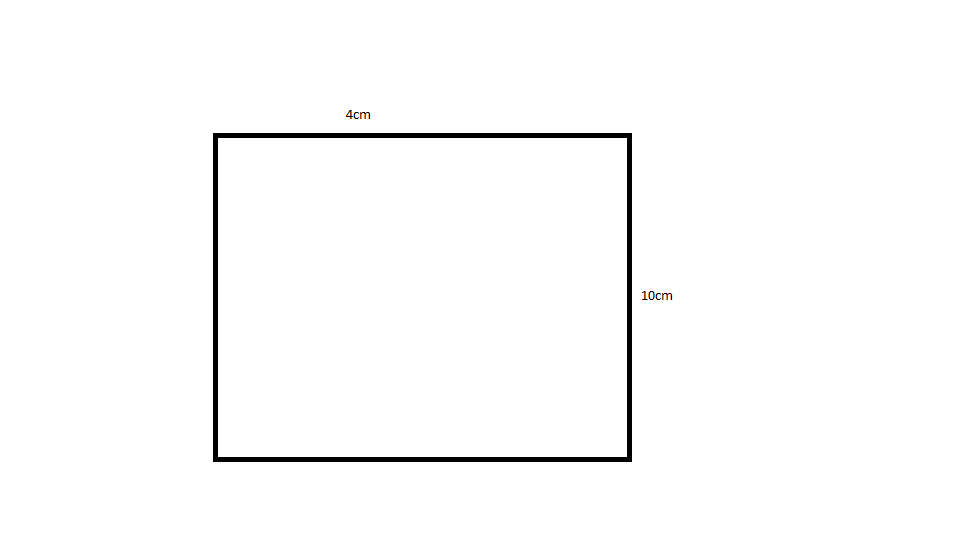
\includegraphics[width=4cm,height=3cm]{media/diagrams/2020/09/14/rectsquare.png}\\\bf{Figure }\bf1.A	
	\end{center}

	
		 &  5 & CO1 & 5\\ \hline
		1.B &
	Derive that iternal sum of angles in an triangle get a sum of 180 degrees \newline
		\begin{center}
		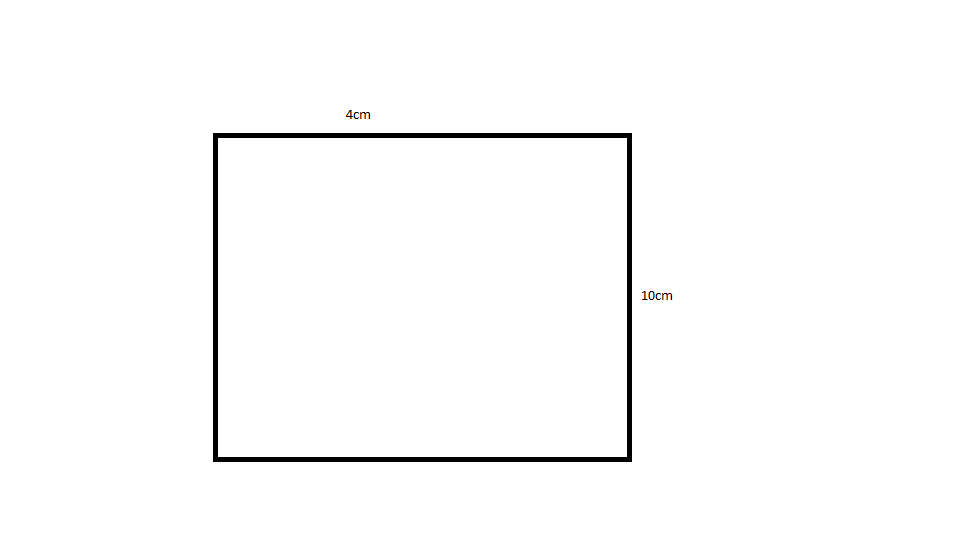
\includegraphics[width=4cm,height=3cm]{media/diagrams/2020/09/14/rectsquare_k3vvwfe.png}\\\bf{Figure }\bf1.B	
	\end{center}

	
		 &  5 & CO1 & 4\\ \hline
		1.C &
	Evaluate $\int x^{3}dx$ \newline
		 &  5 & CO2 & 3\\ \hline
		\end{longtable}

	
	


	
	
		

	
	
	\begin{longtable}{|L{1cm}|L{8cm}|C{1cm}|C{1cm}|C{1cm}|}\hline
			\bf2 & \bf{Attempt} \bf2 out of \bf3 & \bf15 & & \\ \hline
				2.A &
	Evaluate $\frac{x\frac{x}{5}}{dx}$ \newline
		 &  5 & CO1 & 1\\ \hline
		2.B &
	Derive Area of triangle to 1/2 * length*breadth \newline
		 &  5 & CO2 & 6\\ \hline
		2.C &
	Derive the volume of sphere to be 3.14*r*r*r. Where r= radius. \newline
		 &  5 & CO1 & 4\\ \hline
		\end{longtable}

	
	


	
	
		
	
\end{document}